% !TEX spellcheck = en_US
% !TEX spellcheck = LaTeX
%\documentclass[journal,draftcls,onecolumn,11pt,twoside]{IEEEtranTCOM}
\documentclass[11pt, conference, english]{IEEEtran}
%\documentclass[journal,twocolumn,10pt]{IEEEtranTCOM}
\normalsize
\usepackage{lipsum, babel}
%\IEEEoverridecommandlockouts

%\input{header}
\usepackage[cmex10]{amsmath}
\usepackage{%
	amsfonts,%
	amsmath,%
	amssymb,%
	amsthm,%
	%babel,%
	bbm,%
	cite,%
	float,%
	%enumitem,%
	etoolbox,%
	mathrsfs,%
	mathtools,%
	multirow,%
	pgf,%
	pgfplots,%
	subfigure,%
	tikz,%
}
\usepackage[normalem]{ulem}
%\usepackage[vmargin=1.129999cm,hmargin=1cm,head=16pt,includeheadfoot]{geometry}
\usepackage{fancyhdr}
\fancyhead{}
\fancyfoot{}
\fancyhead[LE,RO]{\thepage}
\fancyhead[LO]{\slshape\rightmark}
%\fancyhead[RE]{\slshape\leftmark}
\pagestyle{fancy}

%\tikzset{
%    -|/.style={to path={-| (\tikztotarget)}},
%    |-/.style={to path={|- (\tikztotarget)}},
%}
%\pgfkeys{/pgf/number format/.cd,fixed,precision=3}
%\pgfplotsset{
%	compat=1.3, 
%	every axis/.append style={scale only axis, axis on top,
%		height=4.25cm, width=4.5cm, xmin=-1, xmax=240,
%	}
%}
\usepgflibrary{shapes}
\usetikzlibrary{%
	arrows,positioning, shapes.symbols,shapes.callouts,patterns
}
%\usetikzlibrary{arrows.meta,chains,positioning}
\interdisplaylinepenalty=2500
\theoremstyle{plain}
\newtheorem{thm}{Theorem}%[section]
\newtheorem{lem}[thm]{Lemma}
\newtheorem{prop}[thm]{Proposition}
\newtheorem{cor}[thm]{Corollary}

\theoremstyle{definition}
\newtheorem{defn}[thm]{Definition}
\newtheorem{conj}[thm]{Conjecture}
\newtheorem{exmp}[thm]{Example}
\newtheorem{assum}[thm]{Assumptions}
\newtheorem{axiom}[thm]{Axiom}

\theoremstyle{remark}
\newtheorem{rem}{Remark}
\newtheorem{note}{Note}
\newtheorem{fact}{Fact}

\newcommand{\eq}[1]{\begin{align*}#1\end{align*}}
\newcommand{\EQ}[1]{\begin{equation*}#1\end{equation*}}
\newcommand{\case}[1]{\begin{cases}#1\end{cases}}
\newcommand{\eqn}[1]{\begin{align}#1\end{align}}
\newcommand{\EQN}[1]{\begin{equation}#1\end{equation}}
\newcommand{\meq}[2]{\begin{xalignat*}{#1}#2\end{xalignat*}}
\newcommand{\meqn}[2]{\begin{xalignat}{#1}#2\end{xalignat}}
\newcommand{\ieeeproof}[1]{\begin{IEEEproof}#1\end{IEEEproof}}
\newcommand{\red}[1]{\textcolor{red}{#1}}
\newcommand{\blue}[1]{\textcolor{blue}{#1}}
\newcommand{\green}[1]{\textcolor{green}{#1}}
\newcommand{\norm}[1]{\left\lVert#1\right\rVert}
\newcommand{\indep}{\!\perp\!\!\!\perp}
\DeclarePairedDelimiter\abs{\lvert}{\rvert}%
\newcommand\numberthis{\addtocounter{align}{1}\tag{\thealign}}
\newcommand{\tr}{\operatorname{tr}}
\newcommand{\R}{\mathbb{R}}
\newcommand{\N}{\mathbb{N}}
\newcommand{\E}{\mathbb{E}}
%\newcommand{\mathbb{P}}{\mathbb{P}}
\newcommand{\Z}{\mathbb{Z}}
\newcommand{\B}{\mathscr{B}}
\newcommand{\C}{\mathcal{C}}
\newcommand{\T}{\mathscr{T}}
\newcommand{\F}{\mathcal{F}}
\newcommand{\G}{\mathcal{G}}
\newcommand{\sF}{\mathscr{F}}
\renewcommand{\ge}{\geqslant}
\renewcommand{\le}{\leqslant}
%\newcommand{\ba}{\eq{}
%\newcommand{\ea}{}}
%\DeclareMathOperator*{\argmax}{arg\,max}
\DeclareMathOperator*{\argmax}{arg\,max}
\DeclareMathOperator*{\argmin}{arg\,min}
\renewcommand{\qedsymbol}{$\blacksquare$}

\title{Zero-Shot Learning Using Side Information For Unseen Classes}
\author{
	\IEEEauthorblockN{Sanidhay Bhambay}
	\IEEEauthorblockA{Samsung Electro-Mechanics Software India Bangalore Pvt Limited\\
		\{sanidhay.bhambay\}@samsung.com}% <-this % stops a space
}


\begin{document}
%\lipsum
\markboth{}{SAMSUNG Best Paper Award 2019}

	\maketitle 
	\begin{abstract}
		Inspired from human ability to recognize the unseen objects by just knowing the limited information about it. In learning theory this type of problem is modeled as ``Zero-Shot Learning" (ZSL). In this work we are providing the novel architecture using generative adversarial network (GAN) and dense network to train ZSL model using side information for unseen classes. Our method is able to generate the training instances for unseen classes using GAN by providing the class embedding as an side information input to the generator in GAN. Finally, we have performed our experiments on \textit{Multi Layer Ceramic Captitor} (MLCC) data set to validate our architecture.
		
		
		
		
		
		
%		Zero-shot learning consists of classifying the objects of unseen classes which were not present during training. In this, objects of each class are first map to the semantic feature embedding space. Many sophisticated approaches have been studied in literature for doing this mapping. We are providing an unsupervised way of learning this mapping using auto-encoder architecture in deep learning. Further, for each class, we are converting the class label into a vector containing the set of attributes describing fundamental properties required for the identification of particular class. In last, for assigning the class label for seen and unseen classes in test dataset we are using combination of clustering and nearest neighbor algorithms from machine learning. Clustering is used to avoid brute-force approach for comparing the semantic feature embedding of an object with all attribute vectors of class labels. This approach shown to be outperform the existing comparison methods like $1$-Nearest Neighbor.
		
		
	\end{abstract}
	\begin{IEEEkeywords}
		Deep learning, GAN, MLCC.
	\end{IEEEkeywords}
	\section{Introduction}
	Now a days deep learning is getting more attention in the area where we want to reduce the 
	manual effort by automating the task like manual classification, image captioning etc. Consider the task of image classification,  where training a good deep learning model requires lot of labeled data. However, getting a labeled data for training is expensive and some times not easily available. For example getting sufficient images of endangered species is not easy. Therefore, to handle such cases ZSL~\cite{palatucci2009zero}, gains a lot of attention by researches from last one decade.
	
	
	In ZSL we will be able to label the instances of the classes which were not present during training time. For this each seen/unseen class label is first map to the semantic label space. In natural language processing (NLP) there are techniques to do this like "Skip-Gram Method" or "Google Word2vec". We are using word2vec and CNN-RNN~\cite{scott2016CVPR} based representation to  map each class label to corresponding label space. The main objective in ZSL is to learn the mapping from input space to label space. During the training phase of ZSL, first we have to map the instances of each seen classes to semantic feature space and then map the semantic feature space to label space. The mapping from feature space to label space can be obtained by training a dense neural network.
	
	In this work we first generate the ferature instances for each unseen classes using class embedding from label space as an input to generator in GAN. Remember that during training we are not using any available  data of unseen classes. In contrast, we are generating feature instance of unseen classes using side information from label space. Therefore, our trained model for ZSL is not biased towards only seen classes.
	% before mapping input to corresponding feature space
	
	Several prior work on ZSL is based on learning the mapping from input space to label space and then apply nearest neighbor method to assign the label during test phase~\cite{frome2013devise,lake2011one}. 
	\subsection{Related Work}
In testing phase for an unseen class
object,  the semantic vector is determined by learned mapping and the nearest
neighbor class is assigned~\cite{wang2016relational,socher2013zero}. The most known
approach in ZSL for learning this mapping, is by learning a linear compatibility between the visual and semantic space~\cite{frome2013devise}.
	\subsection{Main Contribution}
	We want to mimic the ability of human to identify unseen object in convolution neural network using ZSL. Apart from prior work which mostly consider the case of learning mapping from input space to label space. In this work we are providing our training model with some side information from label space for unseen classes. For this we are using GAN architecture to generate training instances for unseen classes. In this way we are forcing our model to not biased towards seen classes. Also, we are using Word2vec and CNN-RNN based representaion for class embedding. Finally, we have performed experiments on MLCC data set for both type of class embedding representation.
%	We consider the situation where unseen classes are present in test dataset. Zero-shot learning is the way to deal such practical and potential situation. We are providing a novel unsupervised way of learning object mapping of a particular class to semantic feature embedding space. From deep learning, we are using auto-encoder architecture to learn such mapping. Finally, for assigning class label we are using combination of sophisticated machine learning algorithm called clustering and nearest neighbor which compares the semantic embedding of an object to the attribute vector of the class. 
	\section{Training Phase and Notations}
	In this section, we are going to explain the architecture used during training phase of ZSL and some notations which we are using through out the paper. 
	\subsection{Notations}
	We denote the training set of seen classes by $M=\{(x,y,c(y))|x\in \chi, y \in Y^{s}, c(y) \in C \},$
	where $x\in \mathbb{R}^{d}$ is an feature vector of an image extracted using pre-trained auto-encoder, $y$ denotes the class label from $s$ seen class labels and $c(y)$ denotes the class embedding of class $y$ coming from label space $C$. The class embedding set of unseen classes is denoted by $U=\{(u,c(u))|u \in Y^l,c(u)\in C\},$ where $u$ denotes the class label  from $l$ unseen class label disjoint from $s$ seen class label and $c(u)$ is class embedding of unseen class $u$. For unseen class set we don't have any image feature vector available. Finally we want to learn the mapping,
	$F:\chi \rightarrow Y^s \cup Y^l$.
	 
	
	\subsection{Training Phase}
	In this work we are doing sequential training with GAN followed by dense neural network as shown in Fig.\ref{Fig:SystemModel}. Next, we are going to explain the each component of training phase in detail.
%		\begin{figure}[h!]
%			\centering
%			\scalebox{0.4}{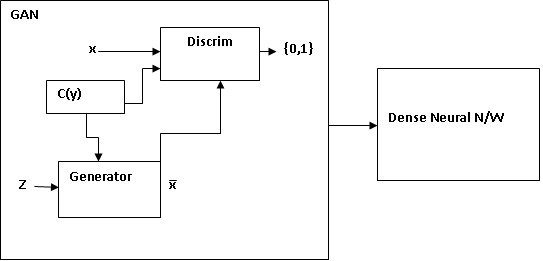
\includegraphics{Figures/Untitled}}
%			\caption{System model used for zero-shot learning.}
%			\label{Fig:SystemModel}
%		\end{figure}
	\subsubsection{Generative Adversarial Network } GAN is used to generate the feature instances of unseen classes. For training GAN we are using only training set $M$ of seen classes. The aim is to learn the generator $G:Z \times C \rightarrow \chi$, where $Z$ is coming from random Gaussian noise. Once the generator learn to generate the feature instance $\bar{x}$ of seen classes, it can also generate the feature instances for unseen classes by passing corresponding class embedding $c(u)$ of unseen classes. In GAN we are going to optimize the following loss function of two player game,
	\eq{\min_G \max_D Loss_{GAN}&=\E [\log D(x,c(y))]\\
		&+\E[\log(1-D(\bar{x},c(y)))],}
	where $\bar{x}=G(z,c(y))$ and $D:\chi \times C \rightarrow [0,1]$ is the discriminator mapping to fake or real.
	\subsubsection{Dense Network}
	 Once the GAN is trained on set $M$, we can generate now the feature instance for unseen classes. Now we have synthetic data for unseen classes denoted by 
	$U=\{(\bar{x},u,c(u))\}$. Finally we have feature instances for seen and unseen classes without using images of unseen classes. Next step is to learn the mapping from input feature space to corresponding label space. For this we are using dense neural network with loss function,
	$Loss_{dense}=\norm{\hat{c}(y)-c(y)}_2,$
	where $\hat{c}(y)$ is the estimate of $c(y)$ at the output layer of dense network. 
	%With this learned dense network we are actually try to find the connection between to two different spaces which is further helpful in assigning labels during test phase.
	
	\section{Testing Phase for ZSL}
	During test phase, first the feature is extracted using pre-trained auto encoder for any query image from unseen classes. Then the extracted feature for this query image is given as an input to dense network. The output of dense network is the class embedding for input query image. In last  nearest neighbor is used between class embedding of query image and class embeddings of all unseen classes. Every class embedding in label space has associated label with that. Therefore, corresponding label is assigned after the search of nearest neighbor.
	\section{Experimental Setup and Evaluation criteria}
	For experiments we are using MLCC data containing $7$ defects classes. Out of $7$ classes we are using $4$ seen classes and $3$ unseen classes. Each class contain images of size $200 \times 128$. For evaluation first we calculate the average accuracy of each unseen class and the taking the average for all unseen classes this evaluation criteria is usually called Top-1 accuracy~\cite{scott2016CVPR}. For class embedding we are using Word2vec and word base CNN-RNN architecture from~\cite{scott2016CVPR}.
	\section{conclusion}
	 In zero-shot learning we are providing the side information to generate the feature instances for unssen classes. Combination of GAN and dense network is used for training phase. During test phase, we are using nearest neighbor algorithm for assigning class labels. Finally, experiments are performed on MLCC data set.
		
%		For application respect, there are various ongoing projects at Samsung, where one needs to classify images depending on the type of defects available in image data. As of now, one needs to re-train their model, whenever Samsung obtains images for the new unseen classes. Zero-shot learning is a useful technique to reduce the manual efforts require for re-training. One just needs to obtain the label attribute vectors for images of unseen classes. 
%	Feature representations can be created for such data, with pre-trained model and ultimately label mapping can help to correctly classify such data.
	
%	

%	\subsection{Auto-Encoder}
%	Auto-encoder used for mapping input object to the semantic feature space of $d$ dimensions is shown in Fig.~\ref{Fig:SystemModel2}. This is an unsupervised way of learning weights of the network. Auto-encoder tries to learn an approximation to the input object, so as to output $\hat{M}_j$ which is very much similar to $M_j$.  The cost function used to get the optimal weights of network is given by,  \eq{J=\sum\limits_{j=1}^{L} Loss\{M_j,\hat{M}_j\},} 
%	where $L$ is the number of data points in the training dataset. The semantic feature embedding $X_j$, for input $M_j$, is obtained as an output of the encoder.
%	
%	\subsubsection{Encoder}
%	An encoder converts the input object into better encoded semantic feature representation $X_j$.
%	We have designed the encoder using convolution neural network (CNN).
%	The feature representation $X_j$ is the encoder's last layer output. Instead of classifying a data, it tries to learn the better way to represent a data with unsupervised way of learning such as dimensionality reduction.
%	
%	\subsubsection{Semantic Feature Embedding}
%	A semantic feature embedding space $F^d$ of $d$ dimensions is a metric space, in which each of the $d$ dimensions represent the relevant feature of input object.
%
%	
%	
%	\begin{figure}[h!]
%		\centering
%		\scalebox{.5}{\begin{tikzpicture}[
font=\large,
draw=black, line width=1pt, >=stealth', node distance=9em,auto,>=latex',
pre/.style={<-,shorten >= 3pt,>=stealth',thick},
post/.style={->,shorten >=1pt,>=stealth',thick},
endState/.style={circle, inner sep=0pt, minimum size=3em},
channel/.style={rectangle,draw,rounded corners, inner sep=0pt, minimum height=6em, minimum width=6em},
intState/.style={rectangle,draw,rounded corners, inner sep=0pt, minimum height=4em, minimum width=8em},
L/.style = {draw, rounded corners},
]
\node [endState] (source) {Original i/p};
\node [intState, right of=source] (encoder) {Encoder}
edge[pre] node[midway,above]{$M_j$} (source);
\node [intState,  right of=encoder](channel) {Feature $``X_j"$}
%edge[pre,|-] node [midway,above] {$X^{n}_j$} (encoder);
edge[pre] node[midway,above]{} (encoder);

\node [intState,  right of=channel] (decoder) {Decoder}

edge[pre] node[midway,above]{} (channel);	 

\node [endState, right of=decoder] (monitor) {Re-Cons i/p}
edge[pre] node[midway,above]{$\hat{M}_j$} (decoder);


\end{tikzpicture}}
%		\caption{Architecture of auto-encoder}
%		\label{Fig:SystemModel2}
%	\end{figure}
%		\subsubsection{Decoder}
%		%Feature vectors are encoded or condensed representations of the input data. 
%		The decoder actually learns how to decode the  feature $X_j$ in order to find the closest estimate $\hat{M}_j$ of the input object $M_j$.
%	%These vectors are the inputs as they make their way back. 
%		The number of output neurons in particular hidden layer of decoder is same as the number of input neurons in corresponding encoder hidden layer. Further, the decoder works in a reverse way that is every layer of the encoder can be represented as an inverse layer in the decoder.
%		Example, inverse of down sampling layer is up sampling layer. 
%		% way of encoder and tries to reconstruct input data, from the feature vectors.
%	%A decoder is the part that tries to reconstruct the original data.
%	% It requires a second feed-forward network, along with back propagation.
%	\subsection{Label Mapping}
%	Each class label is first manually converted into the vector $\{\alpha_j: j\in (1,\dots,\mathbf{card}(Y))\}$,
%	containing the set of attributes describing fundamental properties needed for class identification. The attribute vector $\alpha_j$ of the class label $j$ is of dimension $d$. After clustering, we are employing nearest neighbor or Euclidean distance metric for comparing class attribute vector with the semantic feature vector $X_j$ of the object. A class label $y\in Y$ is assigned to an input object as,
%	\eq{y=\argmin_l \norm{X_j-\alpha_l}_2.}
%	\section{Benefits of Zero-Shot Learning}
%In machine learning, there are various classical classification algorithms like logistic regression, SVM, neural networks etc. During the training phase, these algorithms require label data for each class. Further, they are unable to assign the correct class label of unseen classes present in the test dataset.
%Zero-shot learning overcomes the drawbacks present in above machine learning approaches, by correctly assign the labels of unseen classes in test dataset.
%	% to the test data of new class.
%	\section{Conclusion}
%	We considered a problem of zero-shot learning for classifying objects of unseen classes present in the test dataset. Using auto-encoder architecture from deep learning, we are able to map objects of each class to corresponding semantic feature embedding. Finally, we are using clustering and nearest neighbor algorithm for assigning class labels.
%	
%	For application respect, there are various ongoing projects at Samsung, where one needs to classify images depending on the type of defects available in image data. As of now, one needs to re-train their model, whenever Samsung obtains images for the new unseen classes. Zero-shot learning is a useful technique to reduce the manual efforts require for re-training. One just needs to obtain the label attribute vectors for images of unseen classes. 
	%Feature representations can be created for such data, with pre-trained model and ultimately label mapping can help to correctly classify such data.
	
	
	
	
	
	%%%%%%%%%%%%%%%%%%%%%%%%%%%%%%%%%%%%%%%%%%%%%%%%%%
	\bibliographystyle{IEEEtran}
	\bibliography{document}

	%%%%%%%%%%%%%%%%%%%%%%%%%%%%%%%%%%%%%%%%%%%%%%%%%%%
\onecolumn
\section{Evaluation Criteria and Self Evaluation}
\begin{enumerate}
	\item \textbf{Technological Importance} (30\%)\\
	%1. Technological Importance (30%)
	Is the work about the world's first or an advanced technology?\\
	Does the paper explain and discuss outstanding results? \\
	\textit{\blue{Yes, the paper discusses about a quite frequent issue faced in learning community.}}
	
	\item \textbf{Originality} (30\%)\\
	Does the paper suggest an interesting and creative idea?\\
	Does the paper point out differences or new approaches from related researches?\\
	\textit{\blue{In this paper we have novelty in terms of new system architecture for zero-shot learning.}}
	\item \textbf{Evidences} (30\%)\\
	Does the paper back up a theoretical idea, conclusion, analysis in the literature with sufficient experimental evidences?\\
	Are the conclusions logically consistent and do you logically integrate the issue with the conclusion?\\
	\textit{\blue{Yes, we have sufficient experimental evidence and theoretical ideas to prove that our architecture is reasonably good as compared to existing work.}}
	\item \textbf{Contribution and Impact} (10\%)\\
	Does the conclusions, implications, or outcomes of the paper make some contribution to either the application or the solution itself in the relevant field?\\
	\textit{\blue{Our solution is very much relevant to the problem related to classification and many supervised learning cases.}}
	
	
	
\end{enumerate}
%\lipsum[3]	
%\newpage
%\section{Evaluation Criteria & Self Evaluation}
\end{document}\grid




%1. Paragraph A (Related Work) is isolated; reading flow is abrupt

%
%3. Also, it could be worth to mention about the possible application of ZSL and also, it would be great if we can map application of ZSL for SEMCO/Samsung problems.
%
%4. Highlight the benefit of ZSL over other ML techniques.

